\section{Recursos rítmico-melódicos}
\begin{tcbinformation} 
\textbf{Ideia musical:}
\index{Música!Ideia musical}
\label{ref:ideiamusical}
É uma melodia pequena e muito simples  que não contem recheio né redundâncias obvias \cite[pp. 12]{howard1991aprendendo},
uma ideia pode virar facilmente num \hyperref[sec:Motivo]{\textbf{motivo}} ou uma \hyperref[sec:Frase]{\textbf{frase}},
 se este cumpre com suas respetivas definições.
\end{tcbinformation} 

Para dar maior interesse e apresentar sobre novas formas uma ideia musical, 
existem vários recursos rítmico e melódicos.
Nas seguintes subseções serão apresentados  um listado dos recursos mais comumente usados,
com este fim é usado como origem a ideia musical mostrada na Figura \ref{ritmo:ideiamusical1}. 
\begin{figure}[H]
\centering
\begin{abc}[name=abc-ideiamusical1,width=0.8\linewidth,options={-O= -c -s 1.5}]
X: 1 % start of header
K: C % scale: C major
M: 2/4 %meter - compasso
V:1 %name="Pauta com clave de fá"   sname="Pauta com clave de fá"
[V:1] G1 E1 G1/2 G3/2| A1 G2 F1|
\end{abc}
\caption{Idéia musical.}
\label{ritmo:ideiamusical1}
\end{figure}

%%%%%%%%%%%%%%%%%%%%%%%%%%%%%%%%%%%%%%%%%%%%%%%%%%%%%%%%%%%%%%%%%%%%%%%%%%%%%%%%
\subsection{Sequencia}
\index{Música!Sequencia}
Uma ideia musical pode ser imediatamente repetida, 
com uma transposição a uma altura maior ou menor 
\cite[pp. 30]{bennett1993elementos} \cite[pp. 763]{apel1969harvard}.

A Figura \ref{ritmo:sequence-ex1} mostra o uso de uma ideia musical,
presentada na Figura \ref{ritmo:ideiamusical1}, numa sequencia ascendente correspondente a um tom.
\begin{figure}[H]
\centering
    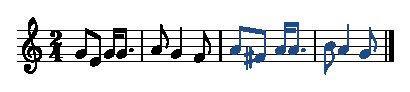
\includegraphics[width=\textwidth]{chapters/cap-musica-composer/sequence-ex1-1.eps}
\caption{Sequencia a partir de uma ideia musical.}
\label{ritmo:sequence-ex1}
\end{figure}

%%%%%%%%%%%%%%%%%%%%%%%%%%%%%%%%%%%%%%%%%%%%%%%%%%%%%%%%%%%%%%%%%%%%%%%%%%%%%%%%
\subsection{Inversão : Reflexão sobre um eixo vertical}
\label{subsec:inversaovertical}
\index{Música!Inversão}

Uma ideia musical pode ser invertida, é dizer escrita ao contrario ao redor de um ponto de pivote;
de modo que as notas com altura descendente passam a ser ascendente, e vice-versa
\cite[pp. 30]{bennett1993elementos}.

A Figura \ref{ritmo:invert-ex1} mostra a inversão, ao redor da nota ``dó'', 
da ideia musical apresentada na Figura \ref{ritmo:ideiamusical1}.
\begin{figure}[H]
\centering
    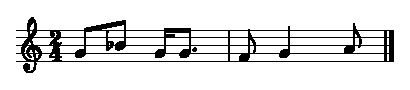
\includegraphics[width=0.8\textwidth]{chapters/cap-musica-composer/invert-ex1-1.eps}
\caption{Inversão de uma ideia musical.}
\label{ritmo:invert-ex1}
\end{figure}


%%%%%%%%%%%%%%%%%%%%%%%%%%%%%%%%%%%%%%%%%%%%%%%%%%%%%%%%%%%%%%%%%%%%%%%%%%%%%%%%
\subsection{Retrogradação : Reflexão sobre um eixo horizontal}
\index{Música!Retrogradação}

Uma ideia musical pode ser escrita em sentido inverso, 
é dizer esta é rescrita iniciando desde a última nota ate a primeira em sequencia contraria 
\cite[pp. 77]{arbones2012armonia}.

A Figura \ref{ritmo:retrogrado-ex1} mostra a retrogradação
da ideia musical apresentada na Figura \ref{ritmo:ideiamusical1}.
\begin{figure}[H]
\centering
    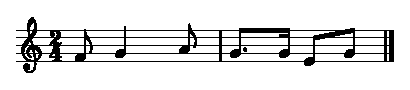
\includegraphics[width=0.8\textwidth]{chapters/cap-musica-composer/retrogrado-ex1-1.eps}
\caption{Retrogradação de uma ideia musical.}
\label{ritmo:retrogrado-ex1}
\end{figure}


%%%%%%%%%%%%%%%%%%%%%%%%%%%%%%%%%%%%%%%%%%%%%%%%%%%%%%%%%%%%%%%%%%%%%%%%%%%%%%%%
\subsection{Diminuição}
\index{Música!Diminuição}

Uma ideia musical pode ser diminuida, é dizer escrita com durações menores
\cite[pp. 30]{bennett1993elementos}.

A Figura \ref{ritmo:diminuicao-ex1} mostra a diminuição, pela divisão entre dois das durações, 
da ideia musical apresentada na Figura \ref{ritmo:ideiamusical1}.
\begin{figure}[H]
\centering
    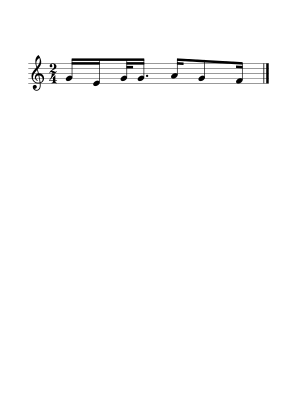
\includegraphics[width=0.8\textwidth]{chapters/cap-musica-composer/diminuicao-ex1-1.eps}
\caption{Diminuião de uma ideia musical.}
\label{ritmo:diminuicao-ex1}
\end{figure}

%%%%%%%%%%%%%%%%%%%%%%%%%%%%%%%%%%%%%%%%%%%%%%%%%%%%%%%%%%%%%%%%%%%%%%%%%%%%%%%%
\subsection{Aumentação}
\index{Música!Aumentação}

Uma ideia musical pode ser aumentada, é dizer escrita com durações maiores
\cite[pp. 30]{bennett1993elementos}.

A Figura \ref{ritmo:aumentacao-ex1} mostra a aumentação, pelo incremento por dois das durações, 
da ideia musical apresentada na Figura \ref{ritmo:ideiamusical1}.
\begin{figure}[H]
\centering
    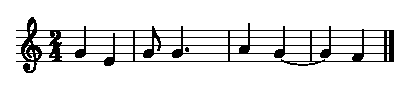
\includegraphics[width=0.8\textwidth]{chapters/cap-musica-composer/aumentacao-ex1-1.eps}
\caption{Aumentação de uma ideia musical.}
\label{ritmo:aumentacao-ex1}
\end{figure}

%%%%%%%%%%%%%%%%%%%%%%%%%%%%%%%%%%%%%%%%%%%%%%%%%%%%%%%%%%%%%%%%%%%%%%%%%%%%%%%%
\subsection{Decoração}
\index{Música!Decoração}

Uma ideia musical pode ser decorada, é dizer podem ser acrescentadas notas ou ornamentos
\cite[pp. 30]{bennett1993elementos}.

A Figura \ref{ritmo:decoracao-ex1} mostra a decoração, pelo aumento de apojaturas e uma linha de expressão, 
na ideia musical apresentada na Figura \ref{ritmo:ideiamusical1}.
\begin{figure}[H]
\centering
    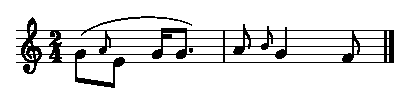
\includegraphics[width=0.8\textwidth]{chapters/cap-musica-composer/decoracao-ex1-1.eps}
\caption{Decoração de uma ideia musical.}
\label{ritmo:decoracao-ex1}
\end{figure}

